\documentclass[addpoints]{exam}
%%%%%%%%%%%%%%%%%% PACKAGES %%%%%%%%%%%%%%%%%%%%%%%%
\usepackage{amsmath}
\usepackage{amsfonts}
\usepackage{tcolorbox}
\tcbuselibrary{skins}
\usepackage{tikz,tkz-euclide,tikz-3dplot}
\usepackage{rotating}
%%%%%%%%%%%%%%%%%%%%%% MARGINS%% %%%%%%%%%%%%%%%%%%%
\extrawidth{.5in}
\extraheadheight{-.25in}
\extrafootheight{-.25in}
%%%%%%%%%%%%%%%%%% ANSWERS AND POINTS %%%%%%%%%%%%%%
%\printanswers
\pointsinrightmargin
\bracketedpoints
%%%%%%%%%%%%%%%%%% HEADER AND FOOTER %%%%%%%%%%%%%%%
\pagestyle{headandfoot}
\firstpageheadrule
\runningheadrule
\firstpageheader{\S4.A.2 Sequences and Series}{}{AP Precalc\\Mr. Carey}
\runningheader{\S4.A.2 Sequences and Series}{}{Mr. Carey}
\firstpagefooter{}{}{}
\runningfooter{ }{\thepage}{ }
%%%%%%%%%%%%%%%%%%%%%% NOTES %%%%%%%%%%%%%%%%%%%%%%%

%%%%%%%%%%%%%%%%%% DOCUMENT CONTENTS %%%%%%%%%%%%%%%
\begin{document}
\section*{Infinite Series}
\subsection*{Investigation 1}
Consider the large box below. With a pen or pencil, cut the box in half and shade one of the two resulting halves. Now, cut the remaining half in half and shade one of the two resulting quarters. Continue this process indefinitely. 
\begin{center}
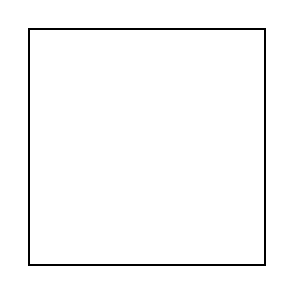
\begin{tikzpicture}
    \draw[thick] (0,0) rectangle (3,3);
\end{tikzpicture}
\end{center}
Consider the following questions:
\begin{questions}
    \question How many times can this process be repeated?
    \question As we continue to make more and more shaded regions, what happens to the area of each new shaded region?
    \question What is the total area of all the shaded regions? Does this total area have a finite value?
\end{questions}

\vspace{\stretch{1}}

\noindent Now repeat this process again, but this time, alternate shading and unshading each half region. What can we say about the total area of all the shaded regions now?
\begin{center}
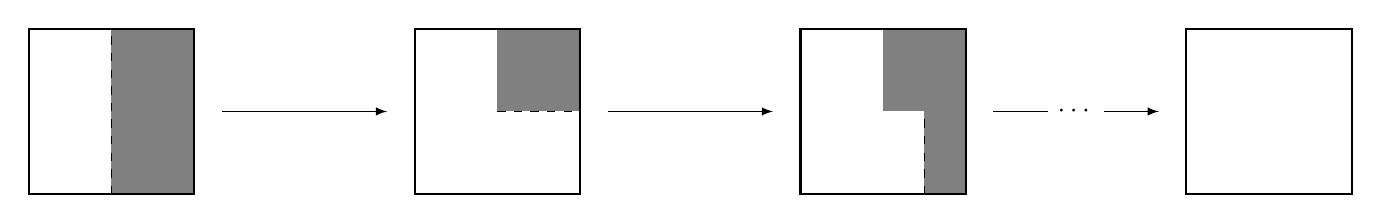
\begin{tikzpicture}[scale=.7]
    \fill[white] (0,0) rectangle (1.5,3);
    \fill[gray] (1.5,0) rectangle (3,3);
    \draw[dashed] (1.5,0) -- (1.5,3);
    \draw[thick] (0,0) rectangle (3,3);

    \fill[white] (7,0) rectangle (8.5,3);
    \fill[gray] (8.5,0) rectangle (10,3);
    \fill[white] (8.5,0) rectangle (10,1.5);
    \draw[dashed] (8.5,1.5) -- (10,1.5);
    \draw[thick] (7,0) rectangle (10,3);

    \fill[white] (14,0) rectangle (15.5,3);
    \fill[gray] (15.5,0) rectangle (17,3);
    \fill[white] (15.5,0) rectangle (17,1.5);
    \fill[gray] (15.5,1.5) rectangle (17,3);
    \fill[gray] (16.25,0) rectangle (17,1.5);
    \draw[dashed] (16.25,0) -- (16.25,1.5);
    \draw[thick] (14,0) rectangle (17,3);

    \draw[-latex] (3.5,1.5) -- (6.5,1.5);
    \draw[-latex] (10.5,1.5) -- (13.5,1.5);
    \draw[-latex] (17.5,1.5) -- (20.5,1.5)node[midway,fill=white]{$\cdots$};

    \draw[thick] (21,0) rectangle (24,3);

\end{tikzpicture}
\end{center}

\subsection*{Investigation 2}
Consider the sequence of lunch tables surrounded by chairs below. Assume that this sequence continues indefinitely.
\begin{center}
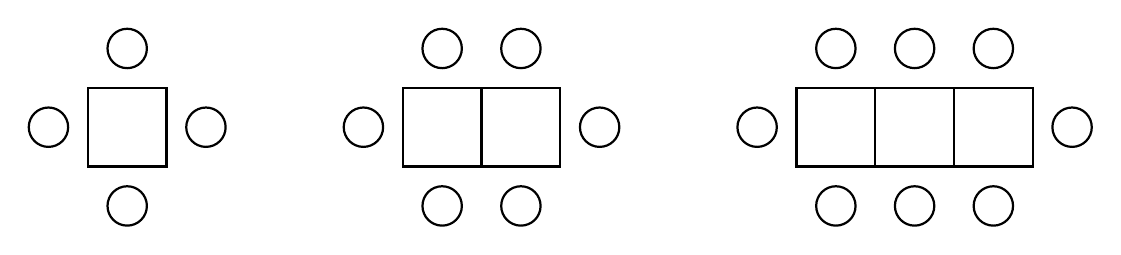
\begin{tikzpicture}
    \draw[thick] (-7,0) rectangle (-6,1);
    \draw[thick] (-7.5,.5) circle (0.25);
    \draw[thick] (-5.5,.5) circle (0.25);
    \draw[thick] (-6.5,1.5) circle (0.25);
    \draw[thick] (-6.5,-.5) circle (0.25);

    \draw[thick] (-3,0) rectangle (-2,1);
    \draw[thick] (-2,0) rectangle (-1,1);
    \draw[thick] (-3.5,.5) circle (0.25);
    \draw[thick] (-.5,.5) circle (0.25);
    \draw[thick] (-2.5,1.5) circle (0.25);
    \draw[thick] (-2.5,-.5) circle (0.25);
    \draw[thick] (-1.5,1.5) circle (0.25);
    \draw[thick] (-1.5,-.5) circle (0.25);

    \draw[thick] (4,0) rectangle (5,1);
    \draw[thick] (2,0) rectangle (3,1);
    \draw[thick] (3,0) rectangle (4,1);
    \draw[thick] (1.5,.5) circle (0.25);
    \draw[thick] (5.5,.5) circle (0.25);
    \draw[thick] (3.5,1.5) circle (0.25);
    \draw[thick] (3.5,-.5) circle (0.25);
    \draw[thick] (2.5,1.5) circle (0.25);
    \draw[thick] (2.5,-.5) circle (0.25);
    \draw[thick] (4.5,1.5) circle (0.25);
    \draw[thick] (4.5,-.5) circle (0.25);
\end{tikzpicture}
\end{center}

\noindent Consider the following questions:
\begin{questions}
    \question Find a formula for the number of chairs needed for the $n$th table.
    \question Find a formula for the total number of chairs needed for the first $n$ tables.
    \question What happens to the total number of chairs as $n$ becomes very large?
\end{questions}

\vspace{\stretch{1}}

\newpage

\begin{tcolorbox}[title=Definition: \textit{Sum of an Infinite Series},title filled,colframe=black,sharpish corners,width=\linewidth]
    The sum of an infinite series is the limit of the sequence of partial sums. If the sequence of partial sums converges to a finite value, then the infinite series is said to \textbf{converge}. 
    \begin{equation*}
        S=\lim_{n\to\infty}S_n=\sum_{i=1}^\infty a_i
    \end{equation*}
    If the sequence of partial sums does not converge to a finite value, then the infinite series is said to \textbf{diverge}.\\

    \noindent\begin{tcolorbox}[enhanced,title=Arithmetic,colback=white,
        colframe=black, colbacktitle=black,inherit height,width=.475\textwidth,attach boxed title to top center=
        {yshift=-3mm,yshifttext=-1mm},
        boxed title style={size=small,colback=gray},nobeforeafter]

        If $a_n$ is an arithmetic sequence, then the sum 
        \[\sum_{i=1}^\infty a_i\]
        is always \textbf{divergent} unless $a_n=0$ for all $n$.
    \end{tcolorbox}\hfill%
    \begin{tcolorbox}[enhanced,title=Geometric,colback=white,
        colframe=black,inherit height,width=.475\textwidth,attach boxed title to top center=
        {yshift=-3mm,yshifttext=-1mm},
        boxed title style={size=small,colback=gray},nobeforeafter]

        If $a_n$ is a geometric sequence, then the sum
        \[\sum_{i=1}^\infty a_i=\frac{a}{1-r}\]
        if $|r|<1$ and diverges otherwise.
    \end{tcolorbox}
\end{tcolorbox}

\subsection*{Examples}
Determine if the sum converges or diverges. If the sum converges, find the value of the sum.
\begin{questions}
    \begin{minipage}{.45\linewidth}
        \question $\displaystyle12+8+4+\cdots$
    \end{minipage}
    \hfill
    \begin{minipage}{.45\linewidth}
        \question $\displaystyle\frac{3}{4}+\frac{1}{2}+\frac{1}{3}+\cdots$
    \end{minipage}

    \vspace{\stretch{.5}}

    \begin{minipage}{.45\linewidth}
        \question $\displaystyle\sum_{k=1}^\infty \frac{1}{15}\cdot\left(\frac{5}{3}\right)^k$
    \end{minipage}
    \hfill
    \begin{minipage}{.45\linewidth}
        \question $\displaystyle\sum_{n=1}^\infty 5n$
    \end{minipage}

    \vspace{\stretch{.5}}

    \begin{minipage}{.45\linewidth}
        \question $\displaystyle 24-12+6-3+\cdots$
    \end{minipage}
    \hfill
    \begin{minipage}{.45\linewidth}
        \question $\displaystyle \sum_{i=3}^\infty4374\left(-\frac{1}{3}\right)^{i-1}$
    \end{minipage}

    \vspace{\stretch{.5}}
\end{questions}

\newpage

\subsection*{Other Examples}

\begin{questions}
    \question A geometric series has a sum of 21 and a first term of 3. Find the common ratio.

    \vspace{\stretch{1}}

    \question Consider the geometric series $\displaystyle\sum_{n=0}^\infty 8\left(\frac{x-1}{3}\right)^n$. For what value(s) of $x$ does the series have a sum?
    
    \vspace{\stretch{1}}
\end{questions}

\section*{Check Your Understanding}

\begin{minipage}[t]{.7\linewidth}
    \subsection*{Questions}
\begin{questions}
    
    \begin{solution}
        \begin{align*}
            6+12\cdot0.6+12\cdot0.6^2+\cdots&=6+12\sum_{n=1}^\infty 0.6^n\\
            &=6+12\left(\frac{0.6}{1-0.6}\right)\\
            &=6+12\left(\frac{0.6}{0.4}\right)\\
            &=6+12(1.5)\\
            &=6+18\\
            &=24
        \end{align*}
    \end{solution}
    \question A geometric series has a sum of 15 and a common ratio of 0.5. Find the first term.
    \question Determine if the series converges or diverges. If the series converges, find the sum.
    \begin{parts}
        \part $\displaystyle\sum_{n=1}^\infty\frac{1}{2^n}$
        \part $\displaystyle\sum_{n=1}^\infty\frac{2^n}{5^2}$
    \end{parts}
    \question A geometric sequence has a 4th term of 16 and a 7th term of 64. Find the sum of the series, if it exists.
    \question A geoemtric sequence has a 3rd term of $-\frac{1}{8}$ and a 6th term of $\frac{1}{64}$. Find the sum of the series, if it exists.
    \question A ball is dropped from a height of 6 feet. Each time the ball bounces, it rebounds to 60\% of the height from which it fell. What is the total vertical distance the ball travels?
\end{questions}
\end{minipage}
\hfill
\begin{minipage}[t]{.25\linewidth}
    
\end{minipage}

\vspace{.2in}


    \rotatebox{180}{\textbf{Answers:}
    1.\, 10\,\,
    2.\,(a) Converges to 1  \,\, (b) Diverges\,\,
    3.\, Diverges\,\,
    4.\, 2/3\,\,
    5.\, 24\,\, \hfill
    }




\end{document}